% Presentazione di laurea — compilare con LuaLaTeX:
%   cd slides && latexmk -lualatex main.tex
\documentclass[aspectratio=169,9pt]{beamer}
\usepackage[italian]{babel}
\usepackage{appendixnumberbeamer}
\usepackage{tema}
\graphicspath{{figure/}}

\title{Stima dei parametri di segnali periodici mediante quantizzazione binaria:}
\subtitle{implementazione e validazione sperimentale dell'algoritmo BQBE}
\author{Othmane Tanta}
\hypersetup{
  pdftitle={Stima dei parametri di segnali periodici mediante quantizzazione binaria: implementazione e validazione sperimentale dell'algoritmo BQBE},
  pdfauthor={Othmane Tanta},
  pdfsubject={Discussione di laurea — Ingegneria Informatica ed Elettronica, Università degli Studi di Perugia},
  pdfkeywords={BQBE, quantizzazione a 1 bit, stima parametrica, Arduino UNO R4}}

\begin{document}

% ============================================================== TITOLO
{\setbeamertemplate{headline}{}
\begin{frame}[plain]
  \centering
  \vspace*{1mm}
  
\includegraphics[height=18mm]{logo_unipg}\par\vspace{1.5mm}
  {\small DIPARTIMENTO DI INGEGNERIA\\CdS in Ingegneria Informatica ed Elettronica}\par
  \vspace{5mm}
  {\color{blutitolo}\LARGE\inserttitle\par\vspace{1mm}\large\insertsubtitle\par}
  \vspace{6mm}
  \begin{minipage}[t]{0.45\textwidth}
    \emph{Candidato}: Othmane Tanta
  \end{minipage}\hfill
  \begin{minipage}[t]{0.45\textwidth}\raggedleft
    \emph{Relatore}: Prof.\ Paolo Carbone
  \end{minipage}
  \vfill
  {\color{blu}\rule{0.8\paperwidth}{0.8pt}}\par\vspace{1.5mm}
  {\small Perugia, Anno Accademico 2025/2026}\par\vspace{1mm}
\end{frame}}

% ============================================================== CONTESTO
\section{Problema e obiettivo}

\begin{frame}{Stima da osservazioni a 1 bit}
  \nota{Contesto: stimare i parametri di un segnale periodico (ampiezza, fase, armoniche)
  usando il convertitore più semplice possibile.}
  \vspace{2mm}

  \begin{columns}[T]
    \begin{column}{0.47\textwidth}
      \centering{\bfseries\color{blu}ADC a $N$ bit}\par\vspace{1mm}
      \begin{tikzpicture}
        \begin{axis}[width=\linewidth,height=34mm,axis lines=left,
            xmin=0,xmax=1,ymin=-1.15,ymax=1.15,xtick=\empty,
            ytick={-1,-0.714,-0.429,-0.143,0.143,0.429,0.714,1},yticklabels={},
            ymajorgrids,grid style={chiaro},
            xlabel={\scriptsize tempo},ylabel={\scriptsize livello},
            xlabel style={at={(1,0)},anchor=north east,inner sep=1pt},
            ylabel style={at={(0,1)},anchor=south,rotate=-90,inner sep=1pt}]
          \addplot[domain=0:1,samples=200,thick,black!70] {sin(deg(2*pi*x))};
          \addplot[const plot,thick,blu,samples=33,domain=0:1]
            {(2*round(3.5*sin(deg(2*pi*x))+3.5)-7)/7};
        \end{axis}
      \end{tikzpicture}\par
      \small campione misurato con $2^N$ livelli\\
      \nota{un ADC flash usa $2^N-1$ comparatori}
    \end{column}
    \begin{column}{0.47\textwidth}
      \centering{\bfseries\color{blu}Quantizzatore a 1 bit: un comparatore}\par\vspace{1mm}
      \begin{tikzpicture}
        \begin{axis}[width=\linewidth,height=34mm,axis lines=left,
            xmin=0,xmax=1,ymin=-1.15,ymax=1.15,xtick=\empty,ytick={0.3},yticklabels={$T$},
            xlabel={\scriptsize tempo},
            xlabel style={at={(1,0)},anchor=north east,inner sep=1pt}]
          \addplot[domain=0:1,samples=200,thick,black!70] {sin(deg(2*pi*x))};
          \addplot[domain=0:1,dashed,magenta,thick] {0.3};
          \addplot[const plot,thick,azzurro,samples=41,domain=0:1]
            {(sin(deg(2*pi*x))>0.3) ? 0.95 : -0.95};
        \end{axis}
      \end{tikzpicture}\par
      \small $y_j = 1$ se $x_j > T$, altrimenti $y_j = 0$\\
      \nota{si conserva solo il \emph{segno} di $x_j - T$}
    \end{column}
  \end{columns}
  \vspace{3mm}

  \centering
  \begin{tikzpicture}[every node/.style={scuro,rounded corners=3pt,minimum height=6mm,text height=1.6ex,text depth=0.3ex}]
    \node[fill=none,text=black] (v) {vantaggi del bit singolo:};
    \node[right=2mm of v] (a) {costo};
    \node[right=2mm of a] (b) {consumo energetico};
    \node[right=2mm of b] {velocità di conversione};
  \end{tikzpicture}\par\vspace{2mm}
  {\bfseries\color{blu}problema:} con un solo bit l'ampiezza sembra persa. Come si ricostruisce il segnale?
\end{frame}

\begin{frame}{Obiettivo della tesi e contributo}
  % TODO: aggiungere il riferimento bibliografico dello stimatore BQBE
  \nota{Punto di partenza: lo stimatore BQBE, che ricava i parametri del segnale dalla
  sola sequenza di bit. Contributo della tesi: portarlo dalla teoria alle misure reali
  e a un microcontrollore.}
  \vspace{3mm}

  \centering
  \begin{tikzpicture}[x=1mm,y=1mm]
    % 1. studio del BQBE
    \node[draw=bordo,thick,minimum width=33mm,minimum height=26mm] at (0,0) {};
    \node[evid,minimum height=8mm,font=\normalsize\bfseries] (b) at (0,0) {BQBE};
    \node[font=\normalsize] (y) at (-12,0) {$y_j$};
    \node[font=\normalsize] (t) at (12,0) {$\hat{\bm\theta}$};
    \draw[freccia] (y) -- (b); \draw[freccia] (b) -- (t);
    % 2. implementazione MATLAB
    \node[tenue,minimum width=33mm,minimum height=26mm,text width=30mm] at (37,0)
      {{\bfseries MATLAB}\\[1mm]pipeline completa\\simulazioni Monte Carlo\\scelta di $\epsilon$ e dei pesi};
    % 3.-4. foto
    \node[inner sep=0pt] at (74,0) {\foto{foto/lab-oscilloscopio.jpg}{33mm}{26mm}};
    \node[inner sep=0pt] at (111,0) {\foto{foto/lab-arduino.jpg}{33mm}{26mm}};
    % linea del tempo
    \foreach \i/\t in {1/{Studio del BQBE},2/{Implementazione MATLAB},3/{Misure reali},4/{Esecuzione su\\microcontrollore}}{
      \node[circle,fill=blu,text=white,font=\small\bfseries,inner sep=1pt,minimum size=5.5mm]
        (c\i) at ({37*(\i-1)},-20) {\i};
      \node[below=1mm of c\i,align=center,font=\small,anchor=north] {\t};
    }
    \foreach \i/\j in {1/2,2/3,3/4} \draw[freccia] (c\i) -- (c\j);
    \draw[decorate,decoration={brace,amplitude=5pt,mirror},thick,azzurro]
      (20,-34) -- (127.5,-34)
      node[midway,below=2mm,font=\small\bfseries,text=blu] {contributo della tesi};
  \end{tikzpicture}
\end{frame}

% ============================================================== METODO
\section{Metodo}

\begin{frame}{Il modello: dal segnale ai bit}
  \[
    x_j = \theta_1 + \sum_{m=1}^{P}\bigl[\theta_{2m}\sin(2\pi m\lambda j)
          + \theta_{2m+1}\cos(2\pi m\lambda j)\bigr]
  \]
  \vspace{1mm}
  \centering
  \begin{tikzpicture}[node distance=5mm,every node/.append style={minimum height=11mm}]
    \node[scuro] (s) {segnale\\$x_j$};
    \node[circle,draw=bordo,fill=chiaro,thick,minimum size=8mm,minimum height=8mm,
          right=of s,inner sep=0pt,font=\bfseries] (p) {+};
    \node[scuro,right=of p] (c) {comparatore\\soglia $T$};
    \node[scuro,right=of c] (b) {bit\\$y_j\in\{0,1\}$};
    \node[evid,right=of b] (e) {stimatore\\BQBE};
    \node[right=4mm of e] (t) {$\hat{\bm\theta}$};
    \node[tenue,below=5mm of p,minimum height=7mm] (r) {rumore $\eta_j\sim\mathcal N(0,\sigma^2)$};
    \draw[freccia] (s) -- (p); \draw[freccia] (p) -- (c); \draw[freccia] (c) -- (b);
    \draw[freccia] (b) -- (e); \draw[freccia] (e) -- (t); \draw[freccia] (r) -- (p);
  \end{tikzpicture}
  \vspace{2mm}

  \begin{columns}[T]
    \begin{column}{0.48\textwidth}
      \[
        p_j = P(y_j = 1) = \Phi\!\left(\frac{x_j - T}{\sigma}\right)
      \]
      \[
        \sigma\,\Phi^{-1}(p_j) = x_j - T
      \]
      \nota{il rumore rende $p_j$ una funzione continua di $x_j$:
      invertendo $\Phi$ si risale al segnale}
    \end{column}
    \begin{column}{0.46\textwidth}
      \begin{tikzpicture}
        \node[tenue,align=left,text width=0.95\linewidth] {%
          \textbf{noti a priori:} $\lambda$, $P$, $\sigma$, $T$\\[1mm]
          \textbf{scelte di progetto:} $N$, $\epsilon$ \ ($H\approx 1/\epsilon$)\\[1mm]
          \textbf{incognite:} $\bm\theta$, $2P+1$ coefficienti};
      \end{tikzpicture}
    \end{column}
  \end{columns}
\end{frame}

\begin{frame}{Lo stimatore BQBE}
  \centering
  \begin{tikzpicture}[node distance=3mm,every node/.append style={minimum height=14mm,text width=24mm,font=\footnotesize}]
    \node[scuro] (a) {\textbf{1. tempi frazionari}\\[1mm]$u_j = \{\lambda j\}\in[0,1)$};
    \node[scuro,right=of a] (b) {\textbf{2. gruppi}\\[1mm]$H$ intervalli di ampiezza $\epsilon$};
    \node[scuro,right=of b] (c) {\textbf{3. probabilità di gruppo}\\[1mm]$\hat p_h = n_{1,h}/n_h$};
    \node[scuro,right=of c] (d) {\textbf{4. linearizzazione}\\[1mm]$Y_h = T + \sigma\,\Phi^{-1}(\hat p_h)$};
    \node[evid,right=of d] (e) {\textbf{5. minimi quadrati pesati}\\[1mm]$\bm Y\approx\bm A\bm\beta\ \to\ \hat{\bm\theta}$};
    \foreach \u/\v in {a/b,b/c,c/d,d/e} \draw[freccia] (\u) -- (\v);
  \end{tikzpicture}
  \vspace{4mm}

  % striscia dei tempi frazionari: pieno = bit 1, vuoto = bit 0
  \begin{tikzpicture}[x=100mm,y=8mm]
    \pgfmathsetseed{7}
    \fill[chiaro] (0,0) rectangle (1,1);
    \foreach \k in {0,...,12} \draw[bordo] (\k/12,0) -- (\k/12,1);
    \draw[bordo,thick] (0,0) rectangle (1,1);
    \foreach \i in {1,...,150}{
      \pgfmathsetmacro{\u}{rnd}
      \pgfmathsetmacro{\v}{0.12+0.76*rnd}
      \pgfmathsetmacro{\pr}{0.5+0.42*sin(deg(2*pi*\u))}
      \pgfmathparse{rnd<\pr ? 1 : 0}
      \ifnum\pgfmathresult=1
        \fill[blu] (\u,\v) circle (0.55mm);
      \else
        \draw[blu,fill=white] (\u,\v) circle (0.55mm);
      \fi}
    \node[below,font=\small] at (0,0) {0};
    \node[below,font=\small] at (1,0) {1};
    \node[right,font=\small] at (1,0.75) {$u_j$};
    \draw[decorate,decoration={brace,amplitude=4pt},thick] (3/12,1.05) -- (4/12,1.05)
      node[midway,above=2pt,font=\small] {$\epsilon$};
    \draw[magenta,very thick] (3/12,0) rectangle (4/12,1);
    \node[font=\small,align=left,anchor=west] at (1.05,0.1)
      {\tikz\fill[blu] circle (0.55mm); bit a 1\\\tikz\draw[blu] circle (0.55mm); bit a 0};
  \end{tikzpicture}
  \vspace{2mm}

  \begin{columns}[T]
    \begin{column}{0.5\textwidth}
      \footnotesize
      \begin{itemize}
        \item nel gruppo le fasi sono vicine: il segnale è quasi costante
        \item[] $\Rightarrow$ si stima \textbf{una sola probabilità per gruppo}, $\hat p_h$
        \item $Y_h \approx \bm a_h^{T}\bm\theta$: $\bm a_h$ contiene $1$, $\sin$ e $\cos$
              delle armoniche valutati sulle fasi del gruppo
      \end{itemize}
    \end{column}
    \begin{column}{0.44\textwidth}
      \begin{tikzpicture}
        \node[tenue,text width=0.93\linewidth,align=left]
          {\textbf{risolvibilità:} servono almeno $2P+1$ gruppi validi, uno per incognita};
      \end{tikzpicture}
    \end{column}
  \end{columns}
\end{frame}

\begin{frame}{Minimi quadrati pesati}
  \begin{columns}[c]
    \begin{column}{0.52\textwidth}
      \centering{\bfseries\color{blu}un sistema sovradeterminato}\par\vspace{2mm}
      \begin{tikzpicture}[font=\small]
        \node[draw=bordo,fill=chiaro,thick,minimum width=5mm,minimum height=22mm] (Y) {$\bm Y$};
        \node[right=1mm of Y] (ap) {$\approx$};
        \node[draw=bordo,fill=blu,text=white,thick,minimum width=16mm,minimum height=22mm,
              right=1mm of ap] (A) {$\bm A$};
        \node[draw=bordo,fill=azzurro,thick,minimum width=5mm,minimum height=13mm,
              right=1.5mm of A] (b) {$\bm\beta$};
        \draw[decorate,decoration={brace,amplitude=4pt,mirror},thick]
          ([xshift=-2mm]Y.north west) -- ([xshift=-2mm]Y.south west)
          node[midway,left=3mm,align=center] {$H$\\gruppi};
        \draw[decorate,decoration={brace,amplitude=4pt}]
          ([yshift=1mm]A.north west) -- ([yshift=1mm]A.north east)
          node[midway,above=2mm] {$2P+1$ incognite};
      \end{tikzpicture}\par\vspace{3mm}
      \small $H$ equazioni $\gg 2P+1$ incognite: nessuna soluzione esatta,\\
      si cerca la $\bm\beta$ che minimizza lo scarto
    \end{column}
    \begin{column}{0.44\textwidth}
      \centering{\bfseries\color{blu}gruppi con affidabilità diversa}\par\vspace{2mm}
      \[
        \bm W = \operatorname{diag}(w_1,\dots,w_H),\qquad w_h = \frac{1}{\operatorname{var}(Y_h)}
      \]
      \begin{tikzpicture}[font=\small]
        \node[draw=bordo,fill=chiaro,thick,minimum size=13mm] (g1) {};
        \foreach \x/\y/\f in {-0.45/0.45/1,-0.15/0.45/1,0.15/0.45/1,0.45/0.45/1,
                              -0.45/0.15/1,-0.15/0.15/1,0.15/0.15/0,0.45/0.15/0,
                              -0.45/-0.15/0,-0.15/-0.15/0,0.15/-0.15/0,0.45/-0.15/0,
                              -0.45/-0.45/1,-0.15/-0.45/0,0.15/-0.45/1,0.45/-0.45/0}{
          \ifnum\f=1 \fill[blu] ($(g1)+(0.8*\x,0.8*\y)$) circle (0.8mm);
          \else \draw[blu,fill=white] ($(g1)+(0.8*\x,0.8*\y)$) circle (0.8mm); \fi}
        \node[draw=bordo,fill=chiaro,thick,minimum size=13mm,right=12mm of g1] (g2) {};
        \foreach \x/\y/\f in {-0.3/0.3/1,0/0.3/1,0.3/0.3/1,-0.3/0/1,0/0/1,0.3/0/1,
                              -0.3/-0.3/1,0/-0.3/1,0.3/-0.3/0}{
          \ifnum\f=1 \fill[blu] ($(g2)+(0.8*\x,0.8*\y)$) circle (0.8mm);
          \else \draw[blu,fill=white] ($(g2)+(0.8*\x,0.8*\y)$) circle (0.8mm); \fi}
        \node[below=1mm of g1,align=center] {$\hat p_h\approx 0.5$\\$w_h$ elevato};
        \node[below=1mm of g2,align=center] {$\hat p_h\approx 1$\\$w_h$ ridotto};
        \fill[azzurro] ($(g1.south)+(-3mm,-17mm)$) rectangle ++(6mm,7mm);
        \fill[azzurro] ($(g2.south)+(-3mm,-17mm)$) rectangle ++(6mm,2mm);
        \draw[bordo,thick] ($(g1.south)+(-9mm,-17mm)$) -- ($(g2.south)+(9mm,-17mm)$);
        \node[left] at ($(g1.south)+(-9mm,-14mm)$) {$w_h$};
      \end{tikzpicture}
    \end{column}
  \end{columns}
  \vspace{1mm}
  \[
    \hat{\bm\beta}_{\text{MQP}} = \arg\min_{\bm\beta}\,(\bm A\bm\beta-\bm Y)^{T}\bm W(\bm A\bm\beta-\bm Y)
    = \bigl(\bm A^{T}\bm W\bm A\bigr)^{-1}\bm A^{T}\bm W\bm Y
  \]
\end{frame}

% ============================================================== ANALISI NUMERICA
\section{Analisi numerica}

\begin{frame}{Verifica della pipeline in MATLAB}
  \centering
  {\color{testotenue}$P=1\quad\cdot\quad N=3000\quad\cdot\quad\sigma=0.5\quad\cdot\quad\epsilon=0.08\quad\cdot\quad T=0$}\par
  \vspace{2mm}
  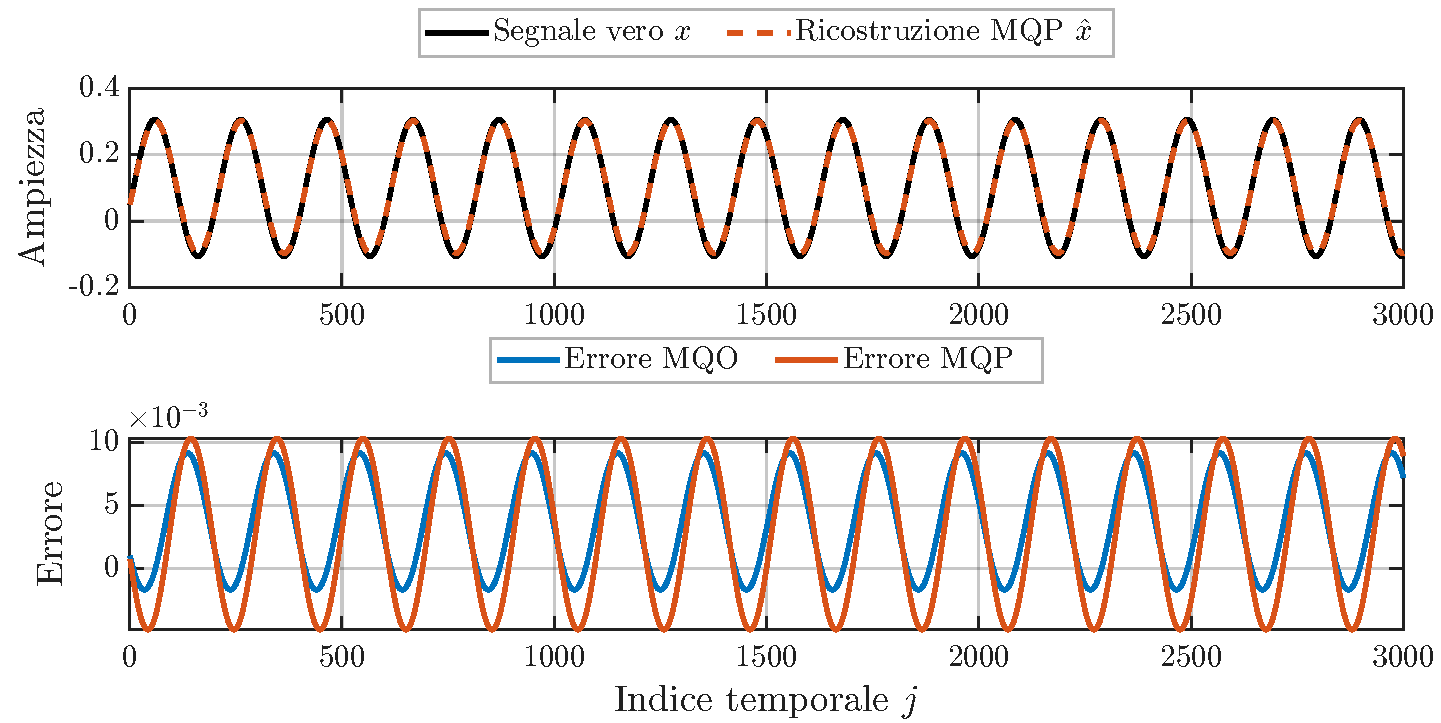
\includegraphics[height=62mm]{verifica_matlab}
\end{frame}

% ============================================================== MISURE
\section{Validazione sperimentale}

\begin{frame}{Banco di misura}
  \centering
  \begin{tikzpicture}[x=1mm,y=1mm,font=\small]
    \tikzset{b/.style={scuro,text width=31mm,minimum height=10mm}}
    % generatore
    \node[tenue,minimum width=76mm,minimum height=22mm,anchor=north west] (g) at (0,0) {};
    \node[anchor=north west,font=\scriptsize\bfseries,text=testotenue] at (g.north west) {Generatore di forme d'onda Keysight 33600A};
    \node[b] (u1) at (19,-13) {Uscita 1 · segnale di prova\\1 kHz · 300 mVpp};
    \node[b] (u2) at (57,-13) {Uscita 2 · rumore gaussiano\\3 Vpp · $B$ = 10 MHz};
    % oscilloscopio
    \node[tenue,minimum width=76mm,minimum height=31mm,anchor=north west] (o) at (0,-30) {};
    \node[anchor=south west,font=\scriptsize\bfseries,text=testotenue] at (o.south west) {Oscilloscopio Teledyne LeCroy · $F_s$ = 100 MSps};
    \node[b,minimum height=6mm,font=\small\bfseries] (c1) at (19,-40) {C1 · riferimento};
    \node[b,minimum height=6mm,font=\small\bfseries] (c2) at (57,-40) {C2 · rumore};
    \node[scuro,text width=69mm,minimum height=6mm,font=\small\bfseries] (f1) at (38,-50) {F1 = C1 + C2 · segnale rumoroso};
    \draw[freccia] (u1) -- (c1); \draw[freccia] (u2) -- (c2);
    \draw[freccia] (c1) -- (c1|-f1.north); \draw[freccia] (c2) -- (c2|-f1.north);
    % PC
    \node[evid,text width=34mm,minimum height=11mm] (pc) at (104,-50) {PC · MATLAB\\quantizzazione a 1 bit, $T$ = 0 V};
    \draw[freccia] (f1.east) -- node[above,font=\scriptsize] {USB} (pc.west);
    \node[below=1mm of pc,align=center,font=\scriptsize] {$\lambda = f_0/F_s = 10^{-5}$ \ · \
      $N = 5\cdot10^{6}$ acquisiti\\stima sui primi $10^{6}$ campioni};
    % foto
    \node[inner sep=0pt,anchor=north] (ph) at (107,0) {\foto{foto/lab-banco.jpg}{52mm}{36mm}};
    \node[below=0.5mm of ph,font=\scriptsize,text=testotenue] {Il banco di misura in laboratorio};
  \end{tikzpicture}
\end{frame}

\begin{frame}{Il rumore: ipotesi e verifica}
  \centering
  \begin{tikzpicture}[font=\small]
    \node[font=\small\bfseries,text=testotenue] at (0,0) {Ipotesi del modello};
    \node[font=\small\bfseries,text=testotenue] at (3.9,0) {Verifica};
    \node[font=\small\bfseries,text=testotenue] at (11.3,0) {Conseguenza};
    \node[scuro,text width=20mm,minimum height=10mm] (a) at (0,-1.7) {rumore\\gaussiano};
    \node (fa) at (3.9,-1.7) {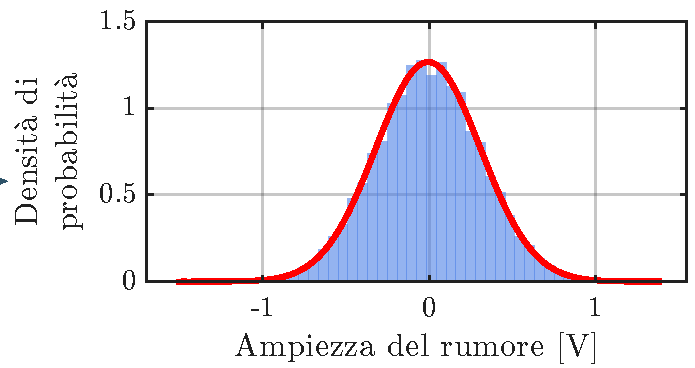
\includegraphics[height=24mm]{rumore_istogramma}};
    \node[align=left,anchor=west] at (6.6,-1.7) {gaussiano \si\\$\sigma\approx 314$ mV};
    \node[scuro,text width=20mm,minimum height=10mm] (b) at (0,-4.6) {campioni\\indipendenti};
    \node (fb) at (3.9,-4.6) {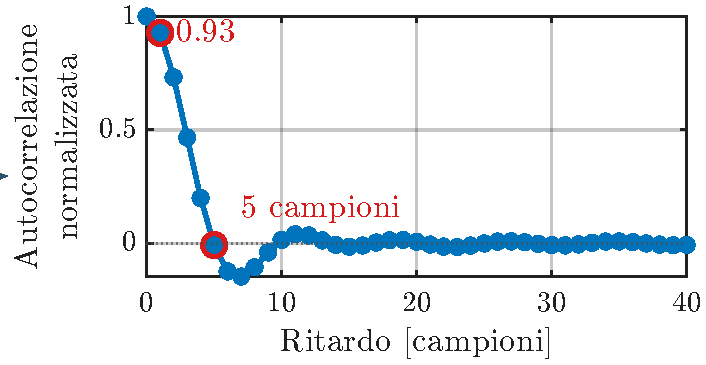
\includegraphics[height=24mm]{rumore_autocorrelazione}};
    \node[align=left,anchor=west] (tb) at (6.6,-4.6) {$\rho(1)=0.93$\\primo zero:\\5 campioni $=1/(2B)$\\campioni correlati \no};
    \node[tenue,text width=22mm] (c1) at (11.3,-4.0) {$\approx N/5$ campioni\\indipendenti};
    \node[evid,text width=26mm,below=3mm of c1] (c2) {decimazione $\times5$:\\da 100 a 20 MSps};
    \draw[freccia] (a) -- (fa.west); \draw[freccia] (b) -- (fb.west);
    \draw[freccia] (tb.east |- c1) -- (c1.west); \draw[freccia] (c1) -- (c2);
  \end{tikzpicture}
\end{frame}

\begin{frame}{Ricostruzione su misure reali}
  \centering
  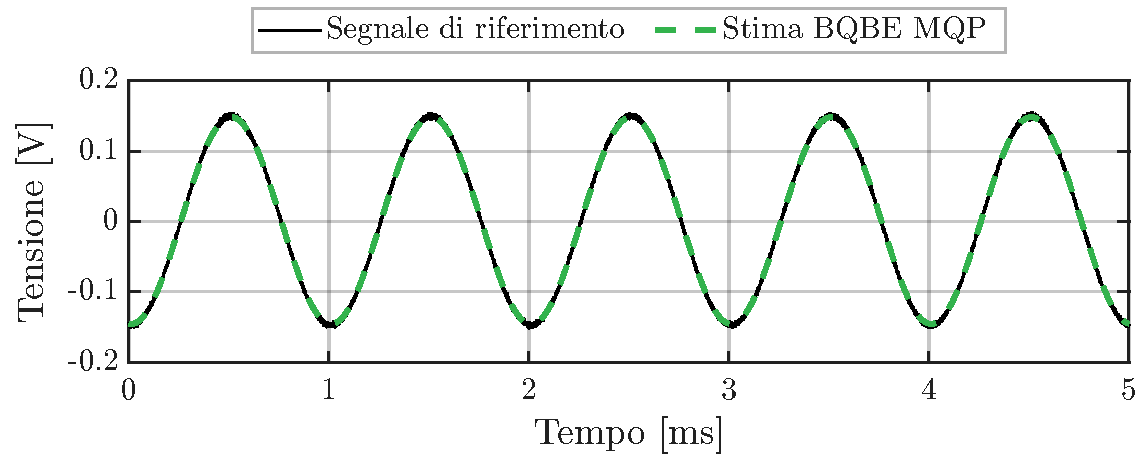
\includegraphics[height=38mm]{ricostruzione_misure}\par\vspace{2mm}
  \begin{columns}[T]
    \begin{column}{0.56\textwidth}
      \footnotesize
      \rowcolors{2}{chiaro}{white}
      \begin{tabular}{@{}lccc@{}}
        \rowcolor{black!80}\color{white}\textbf{Segnale} & \color{white}$\bm{F_s}$ \textbf{[MSps]} &
          \color{white}$\bm N$ & \color{white}\textbf{REQM [V]}\\
        Sinusoide ($P=1$) & 100 & $10^{6}$ & 0.00201\\
        Sinusoide ($P=1$) & 20 & $2\cdot10^{5}$ & 0.00201\\
        Onda triangolare ($P=10$) & 100 & $10^{6}$ & 0.00503\\
        Onda triangolare ($P=10$) & 20 & $2\cdot10^{5}$ & 0.00489\\
      \end{tabular}\par\vspace{1mm}
      \nota{\footnotesize onda triangolare: modello con $P=10$; su Arduino $P=7$ (vincolo di memoria)}
    \end{column}
    \begin{column}{0.4\textwidth}
      \begin{tikzpicture}
        \node[tenue,text width=0.93\linewidth,align=left] {\textbf{decimazione $\times5$:} REQM
        invariata sulla sinusoide, $-2.8\,\%$ sull'onda triangolare\\[1mm]
        $\to$ l'informazione sta nei campioni indipendenti};
      \end{tikzpicture}
    \end{column}
  \end{columns}
\end{frame}

% ============================================================== EMBEDDED
\section{Implementazione embedded}

\begin{frame}{Architettura di validazione}
  \begin{columns}[T]
    \begin{column}{0.52\textwidth}
      \centering
      \begin{tikzpicture}[x=1mm,y=1mm,font=\small]
        \node[evid,text width=62mm,minimum height=7mm] (s) at (0,0) {stessa sequenza binaria $y_j$ \ · \ $N=10^{6}$};
        \node[scuro,text width=29mm,minimum height=19mm,font=\footnotesize] (ar) at (-18,-18) {\textbf{Arduino UNO R4 WiFi}\\C++ · precisione mista\\(float32 + double su $\lambda j$)};
        \node[scuro,text width=29mm,minimum height=19mm,font=\footnotesize] (ml) at (18,-18) {\textbf{MATLAB (riferimento)}\\float64};
        \node[tenue,text width=30mm] (d) at (0,-36) {scarto relativo $\Delta_k$};
        \draw[freccia] (s.south -| ar) -- (ar); \draw[freccia] (s.south -| ml) -- (ml);
        \draw[freccia] (ar.south) -- (d.north -| -8,0); \draw[freccia] (ml.south) -- (d.north -| 8,0);
      \end{tikzpicture}
      \[
        \Delta_k^{(\%)} = \frac{\bigl|\hat\theta_{k,\text{Arduino}}-\hat\theta_{k,\text{MATLAB}}\bigr|}
                               {\bigl|\hat\theta_{k,\text{MATLAB}}\bigr|}\cdot 100
      \]
      \begin{tikzpicture}[font=\footnotesize,every node/.style={tenue,minimum height=7mm}]
        \node (a) {script MATLAB};
        \node[right=1.5mm of a] (b) {firmware Arduino};
        \node[right=1.5mm of b] {libreria C++ BQBE};
      \end{tikzpicture}
    \end{column}
    \begin{column}{0.44\textwidth}
      \centering
      \begin{tikzpicture}[font=\small,x=1mm,y=6.5mm]
        \node[scuro,minimum width=17mm,minimum height=6mm,font=\small\bfseries] (m) at (0,0) {MATLAB};
        \node[scuro,minimum width=17mm,minimum height=6mm,font=\small\bfseries] (a) at (44,0) {Arduino};
        \draw[dashed,bordo] (m.south) -- (0,-6.6);
        \draw[dashed,bordo] (a.south) -- (44,-6.6);
        \foreach \y/\t/\d in {-1/{configurazione della prova}/r,-2/{pacchetto di 256 caratteri}/r,
                              -3/{conferma di ricezione}/l,-4/{pacchetto successivo}/r,-5/{conferma di ricezione}/l}{
          \if\d r\draw[freccia] (0,\y) -- node[above,inner sep=1pt] {\t} (44,\y);
          \else\draw[freccia] (44,\y) -- node[above,inner sep=1pt] {\t} (0,\y);\fi}
        \node at (22,-5.5) {$\vdots$};
        \draw[freccia,very thick] (44,-6.3) -- node[above,inner sep=1pt,font=\small\bfseries] {coefficienti stimati} (0,-6.3);
      \end{tikzpicture}\par\vspace{2mm}
      \nota{seriale USB senza controllo di flusso hardware\\$\to$ controllo di flusso software}
    \end{column}
  \end{columns}
\end{frame}

\begin{frame}{Vincolo di memoria}
  \begin{columns}[T]
    \begin{column}{0.6\textwidth}
      \begin{tikzpicture}
        \node[scuro,minimum width=20mm,minimum height=8mm,font=\normalsize\bfseries] (s) {SRAM 32 kB};
        \node[evid,right=5mm of s,minimum height=8mm,font=\normalsize\bfseries] (b) {budget accumulatori 16\,000 byte};
        \draw[freccia] (s) -- (b);
      \end{tikzpicture}\par\vspace{3mm}
      {\large $M_{\text{acc}} = 8H(1+P)$ byte}\par\vspace{1mm}
      \nota{per gruppo: 2 contatori + $2P$ somme, 4 byte l'una}\par\vspace{2mm}
      \small
      \rowcolors{1}{chiaro}{white}
      \begin{tabular}{@{}l r c l@{}}
        $H=1000,\ P=1$ & 16\,000 B & \si & $\epsilon=10^{-3}$ (= criterio)\\
        $H=1000,\ P=7$ & 64\,000 B & \no & \\
        $H=250,\ P=7$  & 16\,000 B & \si & $\epsilon=4\cdot10^{-3}$ ($\neq$ criterio)\\
      \end{tabular}\par\vspace{3mm}
      {\bfseries\color{blu}con più armoniche, $\epsilon$ è imposto dalla memoria,\\non dalla statistica}
    \end{column}
    \begin{column}{0.37\textwidth}
      \footnotesize
      \riquadro{Elaborazione progressiva}{ogni campione aggiorna il proprio gruppo e viene scartato\\[1mm]
        tempo $\mathcal O(NP)$, memoria $\mathcal O(HP)$, indipendente da $N$}\par\vspace{3mm}
      \riquadro{Precisione mista}{$u_j = \mathrm{float}\bigl(\{\mathrm{double}(\lambda)\cdot\mathrm{double}(j)\}\bigr)$\\[1mm]
        con $j$ fino a $10^6$ la singola precisione altererebbe l'assegnazione al gruppo\\[1mm]
        accumulatori e stima in float32}
    \end{column}
  \end{columns}
\end{frame}

\begin{frame}{Equazioni normali senza la matrice $\bm A$}
  \[
    \bm A^{T}\bm W\bm A = \sum_h w_h\,\bm a_h\bm a_h^{T}
    \qquad\qquad
    \bm A^{T}\bm W\bm Y = \sum_h w_h\,\bm a_h Y_h
  \]
  \vspace{2mm}
  \begin{columns}[T]
    \begin{column}{0.54\textwidth}
      \centering{\small\bfseries\color{testotenue}per ogni gruppo valido $h$}\par\vspace{2mm}
      \begin{tikzpicture}[font=\small,every node/.style={scuro,minimum height=11mm,text width=19mm}]
        \node (a) {costruisci\\la riga $\bm a_h^{T}$};
        \node[right=4mm of a] (b) {accumula nei\\due termini};
        \node[right=4mm of b] (c) {sovrascrivi\\la riga};
        \draw[freccia] (a) -- (b); \draw[freccia] (b) -- (c);
        \draw[freccia] (c.south) -- ++(0,-5mm) -| (a.south);
        \node[fill=none,text=black,text width=,minimum height=0pt,font=\small] at ($(b.south)+(0,-8mm)$) {$h\leftarrow h+1$};
      \end{tikzpicture}
    \end{column}
    \begin{column}{0.42\textwidth}
      \centering{\small\bfseries\color{testotenue}memoria della stima}\par\vspace{2mm}
      \begin{tikzpicture}[font=\small]
        \node[tenue,draw=magenta,text width=45mm] (a) {$\bm A$:\ \ $H\times(2P+1)$\\{\color{magenta}mai memorizzata}};
        \node[evid,text width=45mm,below=2mm of a] {$\bm A^{T}\bm W\bm A$: $(2P+1)\times(2P+1)$\\+ un vettore + una riga};
      \end{tikzpicture}
    \end{column}
  \end{columns}
  \vspace{5mm}
  \begin{tikzpicture}
    \node[tenue,text width=0.95\linewidth,align=left] {\textbf{risoluzione:} eliminazione di Gauss con pivotaggio parziale, nessuna inversa esplicita};
  \end{tikzpicture}
\end{frame}

% ---------------------------------------------------------------- risultati Arduino
% Se è disponibile il grafico della tesi (riferimento + stima Arduino), salvarlo come
% figure/arduino_sinusoide.pdf: sostituisce automaticamente il grafico generato qui.
\begin{frame}{Risultati su Arduino: sinusoide}
  \begin{columns}[c]
    \begin{column}{0.56\textwidth}
      \centering
      \IfFileExists{figure/arduino_sinusoide.pdf}{\includegraphics[width=\linewidth]{arduino_sinusoide}}{%
      \begin{tikzpicture}
        \begin{axis}[width=\linewidth,height=56mm,xmin=0,xmax=5,ymin=-0.2,ymax=0.2,
            xlabel={Tempo [ms]},ylabel={Tensione [V]},grid=major,
            legend style={at={(0.5,1.03)},anchor=south},
            yticklabel style={/pgf/number format/fixed}]
          % stima Arduino, coefficienti della Tabella 4.2 (f0 = 1 kHz)
          \addplot[domain=0:5,samples=400,very thick,dashed,verde]
            {0.001317 - 0.010166*sin(deg(2*pi*x)) - 0.146735*cos(deg(2*pi*x))};
          \addlegendentry{{Stima Arduino ($P=1$, $H=1000$)}}
        \end{axis}
      \end{tikzpicture}}
    \end{column}
    \begin{column}{0.42\textwidth}
      \centering
      \metriche{0.0002\,\%}{$\Delta$ ampiezza}{0.0001\,\%}{$\Delta$ fase}{0.002013 V}{REQM}{57 ms}{fase finale}
      \par\vspace{3mm}
      \scriptsize
      \rowcolors{2}{chiaro}{white}
      \begin{tabular}{@{}lrrr@{}}
        \rowcolor{black!80}\color{white}\textbf{Param.} & \color{white}\textbf{Arduino} &
          \color{white}\textbf{MATLAB} & \color{white}$\bm\Delta$ \textbf{[\%]}\\
        $\hat\theta_1$ & 0.001317 & 0.001317 & 0.0351\\
        $\hat\theta_2$ & −0.010166 & −0.010166 & 0.0024\\
        $\hat\theta_3$ & −0.146735 & −0.146735 & 0.0002\\
        Ampiezza & 0.147087 & 0.147087 & 0.0002\\
        Fase [°] & −93.963196 & −93.963093 & 0.0001\\
      \end{tabular}
    \end{column}
  \end{columns}
  \vspace{3mm}
  \nota{stessa sequenza di bit ($N=10^6$) elaborata da Arduino e da MATLAB · tempo della sola fase finale della stima}
\end{frame}

\begin{frame}{Risultati su Arduino: onda triangolare}
  \begin{columns}[c]
    \begin{column}{0.56\textwidth}
      \centering
      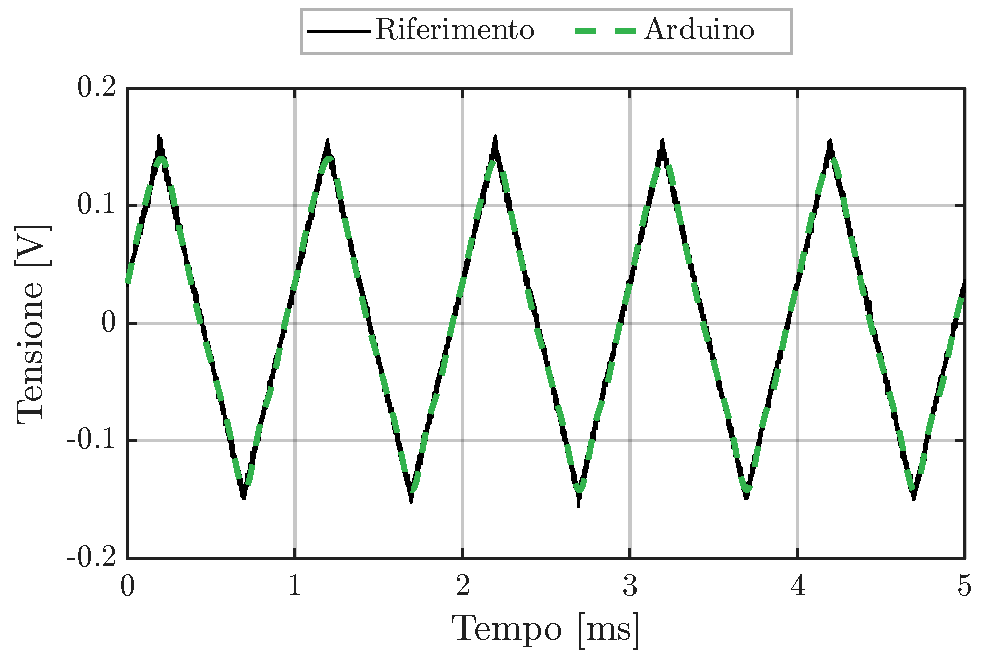
\includegraphics[width=\linewidth]{arduino_triangolare}
    \end{column}
    \begin{column}{0.42\textwidth}
      \centering
      \metriche{0.004557 V}{REQM}{31 ms}{fase finale}{$<3\cdot10^{-7}$}{max $|\Delta|$ assoluto}{15}{coefficienti}
      \par\vspace{3mm}
      \begin{tikzpicture}
        \node[tenue,text width=50mm,align=left,font=\footnotesize] {$P=7$, $H=250$ (vincolo di memoria)\\[1mm]
          scarto relativo massimo $0.28\,\%$ su $\hat\theta_5\approx10^{-4}$: dovuto
          all'arrotondamento a 6 cifre, non all'algoritmo};
      \end{tikzpicture}
    \end{column}
  \end{columns}
  \vspace{3mm}
  \nota{stessa sequenza di bit ($N=10^6$) elaborata da Arduino e da MATLAB · tempo della sola fase finale della stima}
\end{frame}

% ============================================================== CONCLUSIONI
\section{Conclusioni}

\begin{frame}{Conclusioni e sviluppi futuri}
  \begin{columns}[T]
    \begin{column}{0.47\textwidth}
      \begin{tikzpicture}[every node/.style={minimum width=\linewidth,text width=\linewidth-8pt,minimum height=15mm}]
        \node[scuro,minimum height=8mm,font=\normalsize\bfseries] (h) {Conclusioni};
        \node[tenue,align=left,below=3mm of h] (a) {catena BQBE verificata dalla simulazione alle misure reali};
        \node[tenue,align=left,below=2mm of a] (b) {rumore reale gaussiano ma correlato: conta il numero di campioni indipendenti};
        \node[tenue,align=left,below=2mm of b] {BQBE eseguito su Arduino UNO R4};
      \end{tikzpicture}
    \end{column}
    \begin{column}{0.47\textwidth}
      \begin{tikzpicture}[every node/.style={minimum width=\linewidth,text width=\linewidth-8pt,minimum height=15mm}]
        \node[evid,minimum height=8mm,font=\normalsize\bfseries] (h) {Sviluppi futuri};
        \node[tenue,align=left,below=3mm of h] (a) {acquisizione diretta da comparatore e misura del tempo per campione};
        \node[tenue,align=left,below=2mm of a] (b) {piattaforma con più RAM (es.\ STM32) per rispettare il criterio su $\epsilon$ anche con più armoniche};
        \node[tenue,align=left,below=2mm of b] {fattorizzazione di Cholesky sfruttando la simmetria di $\bm A^{T}\bm W\bm A$};
      \end{tikzpicture}
    \end{column}
  \end{columns}
  \vspace{4mm}
  \centering{\color{blutitolo}\large Grazie per l'attenzione}
\end{frame}

% ============================================================== RISERVA
\appendix
\riservatrue
\section{Slide di riserva}

\begin{frame}{$\epsilon$ fisso contro $\epsilon$ adattivo}
  \begin{columns}[c]
    \begin{column}{0.58\textwidth}
      \centering
      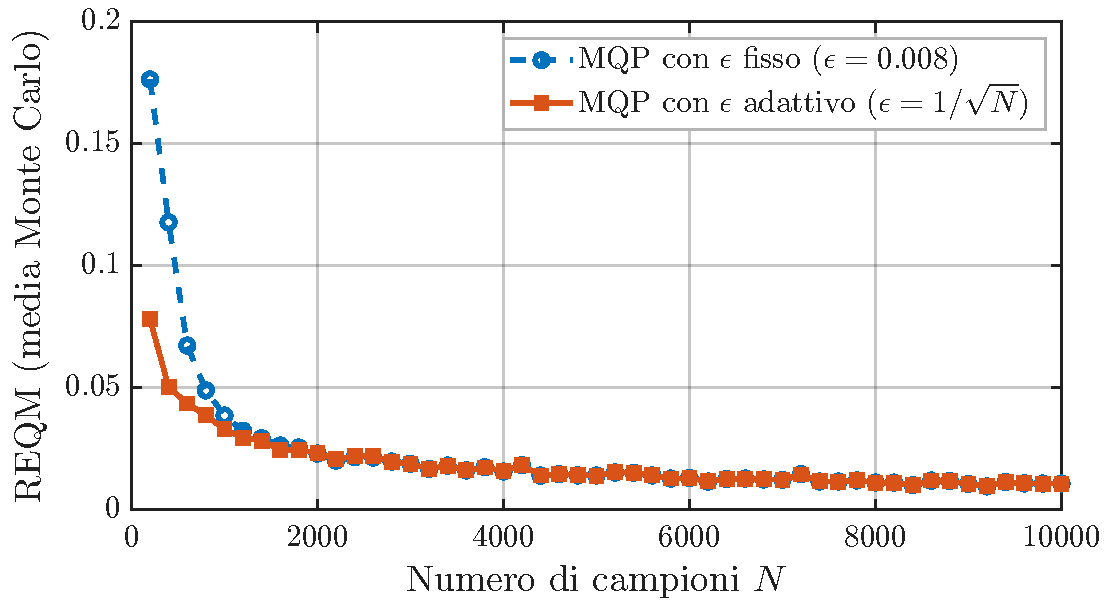
\includegraphics[width=\linewidth]{eps_fisso_adattivo}\par
      {\color{testotenue}$P=1\quad\cdot\quad\sigma=0.5\quad\cdot\quad\epsilon$ fisso $=0.008$}
    \end{column}
    \begin{column}{0.38\textwidth}
      \centering{\bfseries\color{testotenue}criterio adattivo}
      \[
        \epsilon_{\text{opt}} = \min\!\left(\frac{1}{\sqrt N},\ \frac{1}{2P+1}\right)
      \]
    \end{column}
  \end{columns}
\end{frame}

\begin{frame}{Stazionarietà del rumore}
  \centering
  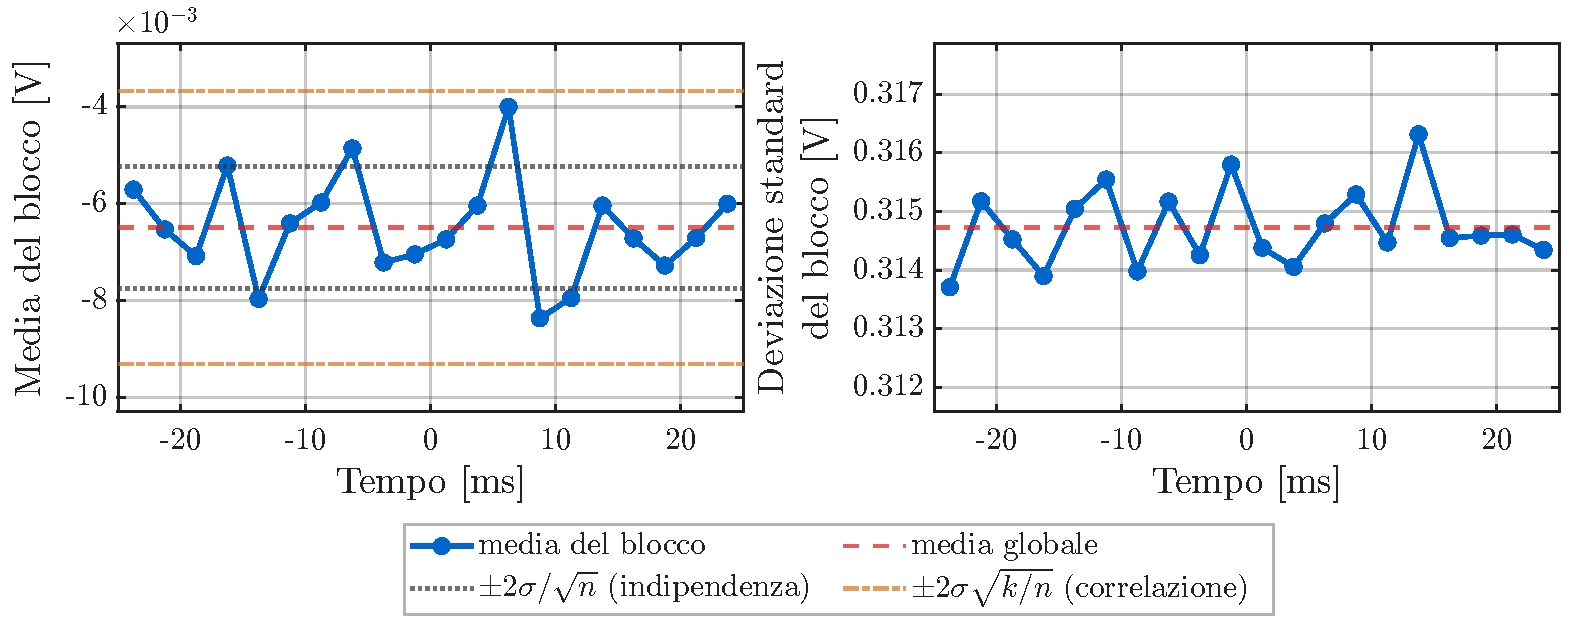
\includegraphics[height=48mm]{stazionarieta_rumore}\par\vspace{2mm}
  \small
  canale C2: $5\cdot10^{6}$ campioni in 20 blocchi \ · \ test classici: rifiuto, perché assumono campioni indipendenti\\
  correggendo per la correlazione (fattore $\approx 4.95$): $\chi^2 = 11.1$ su 19 gradi di libertà ($p\approx0.92$)\\
  deriva della media $1.39\,\%$ di $\sigma$ \ · \ variazione della deviazione standard tra blocchi $0.83\,\%$
\end{frame}

\begin{frame}{Tabelle complete: sinusoide}
  \centering
  \nota{Tabella 4.2: sinusoide ($P=1$, $H=1000$)}\par\vspace{3mm}
  \rowcolors{2}{white}{chiaro}
  \begin{tabular}{@{}lccc@{}}
    \rowcolor{black!80}\color{white}\textbf{Parametro} & \color{white}\textbf{Arduino UNO R4 WiFi} &
      \color{white}\textbf{MATLAB} & \color{white}\textbf{Scarto relativo [\%]}\\
    $\hat\theta_1$ & 0.001317 & 0.001317 & 0.0351\\
    $\hat\theta_2$ & −0.010166 & −0.010166 & 0.0024\\
    $\hat\theta_3$ & −0.146735 & −0.146735 & 0.0002\\
    Ampiezza & 0.147087 & 0.147087 & 0.0002\\
    Fase [gradi] & −93.963196 & −93.963093 & 0.0001\\
  \end{tabular}
\end{frame}

\begin{frame}{Tabelle complete: onda triangolare}
  \centering
  \nota{Tabella 4.3: onda triangolare ($P=7$, $H=250$)}\par\vspace{1mm}
  \scriptsize
  \renewcommand{\arraystretch}{0.95}
  \rowcolors{2}{white}{chiaro}
  \begin{tabular}{@{}lccc@{}}
    \rowcolor{black!80}\color{white}\textbf{Parametro} & \color{white}\textbf{Arduino UNO R4 WiFi} &
      \color{white}\textbf{MATLAB} & \color{white}\textbf{Scarto relativo [\%]}\\
    $\hat\theta_1$ & 0.001132 & 0.001132 & 0.0344\\
    $\hat\theta_2$ & 0.113624 & 0.113624 & <0.0001\\
    $\hat\theta_3$ & 0.041665 & 0.041664 & 0.0015\\
    $\hat\theta_4$ & 0.002571 & 0.002571 & 0.0151\\
    $\hat\theta_5$ & −0.000105 & −0.000105 & 0.2774\\
    $\hat\theta_6$ & −0.008012 & −0.008011 & 0.0131\\
    $\hat\theta_7$ & −0.010821 & −0.010821 & 0.0026\\
    $\hat\theta_8$ & 0.002236 & 0.002236 & 0.0151\\
    $\hat\theta_9$ & 0.000668 & 0.000668 & 0.0339\\
    $\hat\theta_{10}$ & −0.000418 & −0.000418 & 0.0190\\
    $\hat\theta_{11}$ & 0.004494 & 0.004494 & 0.0097\\
    $\hat\theta_{12}$ & −0.001423 & −0.001423 & 0.0239\\
    $\hat\theta_{13}$ & −0.001053 & −0.001052 & 0.0866\\
    $\hat\theta_{14}$ & 0.000375 & 0.000376 & 0.1399\\
    $\hat\theta_{15}$ & −0.002296 & −0.002297 & 0.0397\\
  \end{tabular}
\end{frame}

\end{document}
